\documentclass[11pt]{article}
\usepackage[a4paper,margin=21mm]{geometry}
\usepackage{fontspec}
\setmainfont{Latin Modern Roman}
\newfontfamily\CJKfont{Noto Serif CJK SC}
\XeTeXlinebreaklocale "zh"
\XeTeXlinebreakskip=0pt plus 1pt
\usepackage{amsmath,amssymb,amsthm,amscd,graphicx,color}
\usepackage{xurl}
\usepackage[unicode,hidelinks]{hyperref}
\allowdisplaybreaks
\setlength\emergencystretch{3em}
\numberwithin{equation}{section}

\numberwithin{equation}{section}

\newtheorem{Theorem}{Theorem}[section]
\newtheorem{Corollary}[Theorem]{Corollary}
\newtheorem{Lemma}[Theorem]{Lemma}
\newtheorem{Proposition}[Theorem]{Proposition}
{ \theoremstyle{definition}
\newtheorem{Definition}[Theorem]{Definition}}

\usepackage{mathtools}

\begin{document}
\begin{center}\Large Normalization of the explicit absorbing-wall Macdonald noncolliding-walk kernel for real q and t between zero and one\end{center}
\noindent\textbf{Stable ID:} 1305\quad\textbf{Author:} Leonid Petrov\par
\noindent\textbf{Work:} Noncolliding Macdonald Walks with an Absorbing Wall\par
\noindent\textbf{Source:} \url{https://sigma-journal.com/2022/079/}\par
\noindent\textbf{Version:} Official SIGMA 18 (2022) article 079, DOI 10.3842/SIGMA.2022.079; journal PDF and native TeX acquired 2026-09-30, exact bytes pinned by SHA256\par
\noindent\textbf{Rights:} CC BY 4.0. Authors retain copyright. \url{https://creativecommons.org/licenses/by/4.0/}. Reuse and typesetting adaptation; original language and mathematical content preserved.\par
\noindent\textbf{Difficulty (prior selection preserved):} {\CJKfont H2: The proof encodes a fixed particle configuration as defects in growing partitions and evaluates the principal-specialized branching kernel in that encoding. It separately controls and cancels all large-size powers, coarm/coleg factors, hook products and dual Pieri factors, leaving the specified finite-particle kernel. These asymptotic and telescoping computations establish its normalization from a prior branching rule rather than simply defining a stochastic kernel by renormalization.}\par
\medskip\noindent\textbf{Editorial boundary note (not author text):} Selected full Theorem1.1 sum-to-one kernel for fixed positive m, real0<q,t<1, integer x1>...>xm>=0 and same-chamber y with each yi-xi in\{0,-1\}. Exact formula1.3 and (t,q)-Vandermonde1.1 ordering, full pi/pi-bar maps, principal specialization/branching and complete current Sections3.1–3.7 limiting proof are retained. New powers/coarm/arm-hook/Pieri cancellations, full Proposition3.2 hook-ratio proof and final kernel are unchanged. The author Lemma3.1 says only Straightforward verification; the retained finite coordinate/interlacing step has both exact maps/formulas present, with no editorial expansion. Prior Macdonald branching/principal-specialization/dual-hook identities remain exact cited prerequisites. Absorption/Gibbs/Jack/Hall–Littlewood outcomes receive no counts. Both original panels remain unchanged; literal printed labels have a separate asset-bound editable transcription, with no inferred labels or derived entries.\par
\medskip\hrule\medskip\noindent\textbf{Author text begins below.}\par
\setcounter{section}{1}\setcounter{subsection}{1}
% Original source lines 270--361
\subsection{Macdonald noncolliding walks}\label{sub:intro_details}

Throughout the paper we assume that
$(q,t)$ are real numbers belonging to $(0,1)$.
We need some notation.
Recall that the $q$-Pochhammer symbols are given by
\begin{equation*}
	(z;q)_k\coloneqq (1-z)(1-zq)\cdots\big(1-zq^{k-1}\big),
	\qquad
	k\in \mathbb{Z}_{\ge0},
\end{equation*}
and $(z;q)_\infty\coloneqq\prod_{i=0}^{\infty}(1-zq^i)$ is a convergent infinite
product because $|q|<1$.

For $\vec{\mathsf{x}}=(\mathsf{x}_1>\dots>\mathsf{x}_m\ge0 )$,
denote the $(t,q)$-deformed Vandermonde product by
\begin{equation}
	\label{eq:V_tq}
	V_{t,q}(\vec{\mathsf{x}}):=
	\prod_{1\le i<j\le m}
	\frac{\left( q^{j-i-1}t^{\mathsf{x}_i-\mathsf{x}_j-j+i+1};t \right)_{\infty}}
	{(q^{j-i} t^{\mathsf{x}_i-\mathsf{x}_j-j+i+1};t)_{\infty}}.
\end{equation}
When $t=q\to 1$, $V_{t,q}$ turns (after rescaling by a suitable power of $\log q$)
into the
usual Vandermonde
$V(\vec{\mathsf{x}})=\prod_{1\le i<j \le m}(\mathsf{x}_i-
\mathsf{x}_j)$. Moreover,
when $\mathsf{x}_i=\mathsf{x}_{i+1}$ for some $i$,
one readily sees that $V_{t,q}(\vec{\mathsf{x}})$
vanishes.

Let $\mathsf{y}=(\mathsf{y}_1>\dots>\mathsf{y}_m\ge0 )$
be such that
\begin{equation}\label{eq:y_differs_from_x}
	\mathsf{y}_i-\mathsf{x}_i\in \{ -1,0 \}
	\qquad
	\text{for all $1\le i\le m$}.
\end{equation}
Now we can define the main object of the present paper:
\begin{gather}
\Upsilon_m(\vec{\mathsf{x}},\vec{\mathsf{y}})
		\coloneqq
		t^{-\binom m2}	
		\hspace{1pt}
		\frac
		{V_{t,q}(\vec{\mathsf{y}})}
		{V_{t,q}(\vec{\mathsf{x}})}
		\prod_{\substack{1\le i<j\le m
		\\
		\mathsf{y}_{i}=\mathsf{x}_{i}
		,\,
		\mathsf{y}_{j}=\mathsf{x}_{j}-1}}
		\frac{\big(1-t^{i-j+\mathsf{x}_{i}-\mathsf{x}_{j}+1}
		q^{j-i-1}\big)
		\big(1-t^{i-j+\mathsf{x}_{i}-\mathsf{x}_{j}} q^{j-i+1}\big)}
		{\big(1-t^{i-j+\mathsf{x}_{i}-\mathsf{x}_{j}+1} q^{j-i}\big)
		\big(1-t^{i-j+\mathsf{x}_{i}-\mathsf{x}_{j}} q^{j-i}\big)}
		\nonumber\\
\hphantom{\Upsilon_m(\vec{\mathsf{x}},\vec{\mathsf{y}}) \coloneqq}{}
\times\prod_{i\colon \mathsf{y}_i=\mathsf{x}_i}
		t^{\mathsf{x}_i}
		\prod_{i\colon \mathsf{y}_i=\mathsf{x}_i-1}
		\big(t^{m-i}-q^{m-i}t^{\mathsf{x}_i}\big)		.\label{eq:intro_Upsilon}
\end{gather}
From \eqref{eq:y_differs_from_x}
one readily sees that the infinite products in
${V_{t,q}(\vec{\mathsf{y}})}/{V_{t,q}(\vec{\mathsf{x}})}$
cancel out in such a way that
\eqref{eq:intro_Upsilon} is always a rational function of $q$, $t$.
Moreover, for $0<q,t<1$ the quantities \eqref{eq:intro_Upsilon}
are nonnegative.
One of our main results is the sum-to-one identity for the
$\Upsilon_m$'s:
\begin{Theorem}
	\label{thm:Macdonald_noncolliding_intro}
	With the above notation,
	for any $\vec{\mathsf{x}}=(\mathsf{x}_1>\dots>\mathsf{x}_m\ge0 )$
	we have
	\begin{equation*}
		\sum_{
			\substack{\vec{\mathsf{y}}=
			(\mathsf{y}_1>\dots>\mathsf{y}_m\ge0 )
			\\
			\mathsf{y}_i-\mathsf{x}_i\in \left\{ -1,0 \right\}
			\
			\text{for all $1\le i\le m$}
			}
		}
		\Upsilon_m(\vec{\mathsf{x}},\vec{\mathsf{y}})=1.
	\end{equation*}
\end{Theorem}


% Original source lines 377--387
We prove Theorem~\ref{thm:Macdonald_noncolliding_intro}
in Section~\ref{sec:limit_transition}
by obtaining the transition probabilities
$\Upsilon_m(\vec{\mathsf{x}},\vec{\mathsf{y}})$
as a limit of certain
ratios of Macdonald polynomials
evaluated at the principal specializations
$\big(1,t,t^2,\dots,t^{N-1} \big)$, as the number of variables
goes to infinity. The fact that before the limit
these ratios sum to one is equivalent to the branching
rule for the Macdonald polynomials.

\setcounter{section}{1}
% Original source lines 413--711
\section{Review of Macdonald polynomials}\label{sec:macdonald_polynomials}

Here we collect the necessary notation and results
around Macdonald symmetric polynomials.
We follow \cite[Chapter VI]{Macdonald1995}.

\subsection{Definition}\label{sub:Macdonald_polynomials_definition}

Let $N\ge1$.
Macdonald symmetric polynomials $P_\lambda$ in $N$ variables $x_1,\dots,x_N$
are indexed by partitions
$\lambda=(\lambda_1\ge \dots\ge \lambda_N \ge0)$, $\lambda_i\in \mathbb{Z}$,
with $N$ parts. Denote the set of these partitions by~$\mathbb{Y}(N)$.
The $P_\lambda$'s
depend on two parameters $q,t\in[0,1)$. For each fixed
$(q,t)$, they form a~basis in the space of symmetric
polynomials in~$N$ variables when $\lambda$ runs over~$\mathbb{Y}(N)$.
The shortest definition of the
$P_\lambda$'s is through the first Macdonald $q$-difference operator
acting in the~$x_i$'s:
\begin{gather*}
	D_1\coloneqq \sum_{i=1}^{N}
	\biggl( \prod_{1\le j\le N\colon j\ne i}\frac{x_j-tx_i}{x_j-x_i} \biggr)
	T_{q;i},\\ T_{q;i}f(x_1,\dots,x_N )\coloneqq f(x_1,\dots,x_{i-1},qx_i,x_{i+1},\dots,x_N ).
\end{gather*}
The operator $D_1$ preserves the space of symmetric
polynomials in $x_1,\dots,x_N $, and its eigenfunctions
are the Macdonald polynomials
\begin{gather}
	D_1P_\lambda(x_1,\dots,x_N\mid q,t )=
	\bigl( q^{\lambda_1}t^{N-1}+q^{\lambda_2}t^{N-2}+\dots+q^{\lambda_N}
	\bigr)
	P_\lambda(x_1,\dots,x_N\mid q,t ),\label{eq:Macdonald_eigenrelation}
\end{gather}
with $\lambda\in \mathbb{Y}(N)$.
For generic $(q,t)$, the eigenvalues in~\eqref{eq:Macdonald_eigenrelation}
for different $\lambda$ are distinct, so
the $P_\lambda$'s are determined uniquely up to normalization.
The normalization is specified by
\begin{equation*}
	P_\lambda(x_1,\dots,x_N\mid q,t )=
	x_1^{\lambda_1}x_2^{\lambda_2}\cdots x_N^{\lambda_N} +
	\text{lexicographically lower terms},
\end{equation*}
where the lower terms depend on $q$, $t$.

In the case $q=t$, the polynomials $P_\lambda$ reduce to the
well-known Schur symmetric polynomials~$s_\lambda$, which admit
the following explicit determinantal formula (which does not
depend on the choice of $q$):
\begin{equation}
	\label{eq:Schur}
	P_\lambda(x_1,\dots,x_N\mid q,q )=s_\lambda(x_1,\dots,x_N )=
	\frac{\det\bigl[ x_i^{\lambda_j+N-j} \bigr]_{i,j=1}^{N}}{\det
	\bigl[ x_i^{N-j} \bigr]_{i,j=1}^N}.
\end{equation}
For generic $(q,t)$, there are no known formulas for Macdonald polynomials which are as compact as~\eqref{eq:Schur}.

\subsection{Principal specialization}\label{sub:principal_specialization}

\begin{figure}[htpb]
	\centering
	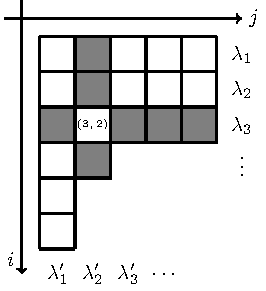
\includegraphics[width=.28\textwidth]{../assets/1305/fig_Young_d.pdf}
	\caption{Young diagram $\lambda=(5,5,5,2,1,1)$. Highlighted
		are the arm, leg, coarm, and coleg of the box $\square=(3,2)$.
		We have $|\lambda|=19$ and
		$a(\square)=3$, $l(\square)=1$, $a'(\square)=1$, $l'(\square)=2$.}
	\label{fig:Young_d}
\end{figure}

When the variables $x_i$ are specialized to a finite geometric
progression with the ratio $t$ (the second Macdonald parameter),
the polynomials $P_\lambda$ admit an explicit product formula in terms
of the Young diagram corresponding to the partition $\lambda$.
Recall that the Young diagram $\lambda$ is a~collection of $1\times 1$ boxes in the plane
with $\lambda_i$ boxes in row $i$, see Figure~\ref{fig:Young_d}
for an illustration.
The principal specialization takes the form
\cite[formulas~(VI.6.11) and (VI.6.11$'$)]{Macdonald1995}:
\begin{equation}	\label{eq:principal_spec}
	P_\lambda\big(1,t,\dots,t^{N-1} \mid q,t \big)=
	t^{n(\lambda)}\prod_{\square\in \lambda}
	\frac{1-q^{a'(\square)}t^{N-l'(\square)}}
	{1-q^{a(\square)}t^{l(\square)+1}},
\end{equation}
where the product is over all boxes of the Young diagram $\lambda$,
\begin{equation}	\label{eq:n_lambda_notation}
	n(\lambda):=\sum_i(i-1)\lambda_i,
\end{equation}
and the arms, legs, coarms, colegs of the box $\square=(i,j)$
are defined, respectively, as
\begin{equation}	\label{eq:arms_legs}
	a(\square)=\lambda_i-j,\qquad l(\square)=\lambda_j'-i,\qquad
	a'(\square)=j-1,\qquad l'(\square)=i-1.
\end{equation}
Here $\lambda_j'$ are the column lengths in the Young
diagram, see Figure~\ref{fig:Young_d}.

\subsection{Branching}\label{sub:branching}

Let us first recall the Pieri coefficients for Macdonald polynomials
\cite[formula~(VI.6.24.ii)]{Macdonald1995},
\cite[formula~(2.11)]{BorodinCorwin2011Macdonald}.
They depend on a pair of partitions $\mu$, $\lambda$
which \emph{interlace}, namely,
\begin{equation*}%\label{eq:interlace}
	\lambda_1\ge \mu_1\ge \lambda_2\ge \mu_2\ge \cdots
\end{equation*}
(notation $\mu\prec \lambda$), and are defined as
\begin{equation}
	\label{eq:psi_Pieri}
	\psi_{\lambda/\mu}
	=
	\psi_{\lambda/\mu}(q,t)
	\coloneqq
	\prod_{1\le i<j\le \ell(\mu)}
	\frac{\mathsf{f}\big(q^{\mu_i-\mu_j}t^{j-i}\big)
	\hspace{1pt}\mathsf{f}\big(q^{\lambda_i-\lambda_{j+1}}t^{j-i}\big)}
	{\mathsf{f}\big(q^{\lambda_i-\mu_j}t^{j-i}\big)
	\hspace{1pt}\mathsf{f}\big(q^{\mu_i-\lambda_{j+1}}t^{j-i}\big)},
	\qquad
	\mathsf{f}(u):=\frac{(tu;q)_{\infty}}{(qu;q)_{\infty}}.
\end{equation}
Here and below by $\ell(\mu)$ we denote the number of
parts in $\mu$ which are strictly positive,
that is, $\mu_{\ell(\mu)}>0$, $\mu_{\ell(\mu)+1}=0$ (when $\mu=(0,0,\dots )$, we set $\ell(\mu)=0$).
Let also $|\lambda|=\lambda_1+\dots+\lambda_{\ell(\lambda)}$
denote the number of boxes in the Young diagram~$\lambda$.

\begin{Proposition}[{\cite[formula~(VI.7.13$'$)]{Macdonald1995}}]
	\label{prop:branching}
	Let $\lambda\in \mathbb{Y}(N)$.
	We have
	\begin{equation}
		\label{eq:branching}
		P_\lambda(x_1,\dots,x_N \mid q,t)
		=
		\sum_{\mu\colon\mu\prec\lambda}
		\psi_{\lambda/\mu}(q,t)\hspace{1pt} P_\mu(x_1,\dots,x_{N-1} \mid q,t )\hspace{1pt}
		x_N^{|\lambda|-|\mu|},
	\end{equation}
	where the sum is over
	$\mu\in \mathbb{Y}(N-1)$ which interlace with $\lambda$.
\end{Proposition}

Note that for $q,t\in [0,1)$ the coefficients $\psi_{\lambda/\mu}$
\eqref{eq:psi_Pieri} are all nonnegative.
Together with Proposition~\ref{prop:branching} this implies:
\begin{Corollary}
	\label{cor:nonnegative_spec}
	Let $q,t\in[0,1)$. Specializing the variables
	$x_1,\dots,x_N $ into
	nonnegative real numbers
	makes the Macdonald polynomial
	$P_\lambda(x_1,\dots,x_N\mid q,t)$ nonnegative.
\end{Corollary}

More generally, for $N\ge K\ge1$
define the skew Macdonald polynomials
$P_{\lambda/\mu}$
as the coefficients
in the expansion:
\begin{equation*}
	P_\lambda(x_1,\dots,x_N \mid q,t)=
	\sum_{\mu\in \mathbb{Y}(K)}
	P_\mu(x_1,\dots,x_K \mid q,t )
	P_{\lambda/\mu}(x_{K+1},\dots,x_{N-1},x_N \mid q,t ).
\end{equation*}
Here we use the fact that
the polynomials
$P_\mu(x_1,\dots,x_K )$
form a basis in the space of symmetric functions in $K$ variables, and
expand
$P_\lambda(x_1,\dots,x_N )$
in this basis.
The Pieri coefficient is related to the skew Macdonald polynomial
in one variable as follows:
\begin{equation*}%\label{eq:P_skew_single_variable}
	P_{\lambda/\mu}(x_1\mid q,t)=
	\begin{cases}
		\psi_{\lambda/\mu}(q,t)\hspace{1pt} x_1^{|\lambda|-|\mu|},&\mu\prec \lambda,\\
		0,&\text{otherwise}.
	\end{cases}
\end{equation*}

Later we will also use the dual Pieri coefficients
$\psi_{\lambda/\mu}'$ which are defined as
(see \cite[formula~(VI.6.24.iv)]{Macdonald1995} and
\cite[formula~(2.12)]{BorodinCorwin2011Macdonald})
\begin{equation}
	\label{eq:psi_prime_Pieri}
	\psi_{\lambda/\mu}'=
	\psi_{\lambda/\mu}'(q,t)
	\coloneqq
	\prod_{\substack{i<j \\ \lambda_{i}=\mu_{i},\, \lambda_{j}=\mu_{j}+1}}
	\frac{\big(1-q^{\mu_{i}-\mu_{j}} t^{j-i-1}\big)\big(1-q^{\lambda_{i}-\lambda_{j}} t^{j-i+1}\big)}
	{\big(1-q^{\mu_{i}-\mu_{j}} t^{j-i}\big)\big(1-q^{\lambda_{i}-\lambda_{j}} t^{j-i}\big)}.
\end{equation}
for partitions $\lambda$, $\mu$ whose column lengths interlace,
that is,
$\lambda_1'\ge \mu_1'\ge \lambda_2'\ge \mu_2'\ge \cdots $.
We have
\begin{equation}
	\label{eq:P_skew_single_variable_dual}
	P_{\lambda'/\mu'}(x_1 \mid t,q)=
	\begin{cases}
		\psi'_{\lambda/\mu}(q,t)\hspace{1pt} x_1^{|\lambda|-|\mu|}
		,&\mu'\prec \lambda',\\
		0
		,&\text{otherwise}.
	\end{cases}
\end{equation}

\subsection{Cauchy identity}\label{sub:Cauchy_and_Dyson1}

Along with the branching rule, another fundamental
identity for Macdonald polynomials is the Cauchy identity.
Here we present its dual version, see \cite[Chapter~VI.4]{Macdonald1995} for the
usual version.

\begin{Proposition}[{\cite[formula~(VI.5.4) and Chapter~VI.7]{Macdonald1995}}]
	\label{prop:dual_Cauchy_identity}
	Let $N,M\ge 1$ be fixed. We have
	\begin{equation*}%\label{eq:dual_Cauchy}
		\sum_{\lambda\in \mathbb{Y}(N)\colon \lambda_1\le M}
		P_\lambda(x_1,\dots,x_N \mid q,t)
		\hspace{1pt}
		P_{\lambda'}(y_1,\dots,y_M\mid t,q )=
		\prod_{i=1}^{N}\prod_{j=1}^{M}(1+x_iy_j).
	\end{equation*}
	Moreover, for any $\mu\in \mathbb{Y}(N)$ we have
	the following particular case of
	the skew Cauchy identity:
	\begin{equation}		\label{eq:dual_Cauchy_skew}
		P_\mu(x_1,\dots,x_N\mid q,t )
		\prod_{i=1}^{N}(1+x_iy)=
		\sum_{\lambda\in \mathbb{Y}(N)\colon \mu'\prec \lambda'}
		P_{\lambda'/\mu'}(y\mid t,q)
		\hspace{1pt}
		P_\lambda(x_1,\dots,x_N\mid q,t ).
	\end{equation}
\end{Proposition}
Identities~\eqref{eq:branching} and~\eqref{eq:dual_Cauchy_skew} look very similar, but note that
in the former we sum over the smaller partition, while in the latter one we sum over the larger partition.

\subsection{Markov kernels from Macdonald polynomials}\label{eq:Markov_kernels_from_Cauchy}

Let us first recall a general definition from
\cite[Chapter~7]{borodin2016representations}.
Let $\mathfrak{X}$, $\mathfrak{Y}$ be
finite or countable sets. By a Markov kernel
(or a link) from $\mathfrak{X}$ to $\mathfrak{Y}$,
we mean a function $P$ on $\mathfrak{X}\times \mathfrak{Y}$
such that
$P(x,y)\in[0,1]$ for all $x\in \mathfrak{X}$, $y\in \mathfrak{Y}$,
and
\begin{equation*}
	\sum_{y\in \mathfrak{Y}}P(x,y)=1
	\qquad
	\text{for all $x\in \mathfrak{X}$}.
\end{equation*}
We adopt the notation $P\colon \mathfrak{X}\dashrightarrow \mathfrak{Y}$.

Normalizing identities
\eqref{eq:branching} and \eqref{eq:dual_Cauchy_skew}
with nonnegative variables $x_i$ and $y$
(following
\cite{Borodin2010Schur,BorFerr2008DF} in the Schur case and~\cite{BorodinCorwin2011Macdonald}
in the general Macdonald case)
leads to the following two families of links:
\begin{align}
\Lambda^{N}_{N-1}\colon \ & \mathbb{Y}(N)\dashrightarrow \mathbb{Y}(N-1),
		\nonumber\\
		& \Lambda^{N}_{N-1}(\lambda,\mu)\coloneqq
		\psi_{\lambda/\mu}(q,t)\hspace{1pt} x_N^{|\lambda|-|\mu|}\hspace{1pt}
		\frac{
		P_\mu(x_1,\dots,x_{N-1} \mid q,t )
		}
		{P_\lambda(x_1,\dots,x_N \mid q,t)}
		\,\mathbf{1}_{\mu\prec\lambda},\label{eq:traditional_links_Lambda}\\
Q_N\colon \ & \mathbb{Y}(N)\dashrightarrow \mathbb{Y}(N),
		\nonumber\\
		& Q_N(\lambda,\nu)\coloneqq
		\frac{\psi'_{\nu/\lambda}(q,t)
		\hspace{1pt}
		y^{|\nu|-|\lambda|}
		}
		{\prod_{i=1}^{N}(1+x_i y)}
		\frac
		{
		P_\nu(x_1,\dots,x_N\mid q,t )}
		{P_\lambda(x_1,\dots,x_N\mid q,t )}
		\,\mathbf{1}_{\lambda'\prec\nu'}		.\label{eq:traditional_links_Q}
\end{align}
Here and
throughout the paper by $\mathbf{1}_{A}$ we denote
the indicator of the event (or condition) $A$.
For the link \eqref{eq:traditional_links_Q}
we also used \eqref{eq:P_skew_single_variable_dual}.

\setcounter{section}{2}
% Original source lines 768--1431
\section{Limit transition to noncolliding walks}\label{sec:limit_transition}

In this section we perform the limit transition as $N\to+\infty$ in the
Markov kernels $\Lambda^{N}_{N-1}$ \eqref{eq:traditional_links_Lambda}
under the principal specialization
\eqref{eq:principal_spec}, and prove
Theorem~\ref{thm:Macdonald_noncolliding_intro}.

\subsection{Setup}\label{sub:limit_transition_setup}

Denote by $\mathbb{W}_m$ the space of $m$-particle configurations
in $\mathbb{Z}_{\ge0}$, that is,
\begin{equation}
	\label{eq:W_m_space}
	\mathbb{W}_m\coloneqq
	\{
		\vec{\mathsf{x}}=(\mathsf{x}_1>\mathsf{x}_2>\dots>\mathsf{x}_m\ge0 )
	\}\subset \mathbb{Z}_{\ge0}^{m}.
\end{equation}
By $\mathbb{W}_m(N)$ denote the finite subset of $\mathbb{W}_m$ determined by
the condition
$\mathsf{x}_1\le N+m-2$. Define the injective maps
\begin{equation}
	\label{eq:pi_maps_1}
	\pi\colon \ \mathbb{W}_m(N)\to \mathbb{Y}(N), \qquad
	\overline\pi\colon \ \mathbb{W}_m(N)\to \mathbb{Y}(N-1),
\end{equation}
as follows. If $\lambda=\pi(\vec{\mathsf{x}})\in \mathbb{Y}(N)$
and $\mu=\overline\pi(\vec {\mathsf{y}})\in \mathbb{Y}(N-1)$, then
\begin{gather}
 \{ \lambda_1-1,\lambda_2-2,\dots,\lambda_N-N \}=
 \{ 0,1,2,\dots,N+m-1 \}\setminus
		\{\mathsf{x}_1,\dots, \mathsf{x}_m \},\nonumber\\
		 \{ \mu_1-1,\mu_2-2,\dots,\mu_{N-1}-(N-1) \}=
		 \{ 1,2,\dots,N+m-1 \}\setminus
		\{\mathsf{y}_1+1,\dots, \mathsf{y}_m+1 \}.\!\!\!\label{eq:pi_maps_2}
	\end{gather}
For fixed $\vec{\mathsf{x}}$ and growing $N$,
almost all parts of $\lambda=\pi(\vec{\mathsf{x}})$
are equal to $N+m$, and there is a defect in a few last parts of
$\lambda$. The columns of this defect are
encoded through
$\vec{\mathsf{x}}$. A similar description holds for
$\mu=\overline\pi(\vec{\mathsf{y}})$.
In multiplicative notation for partitions, we have
\begin{gather}
		\lambda=\pi(\vec{\mathsf{x}})=
		(N+m)^{N-\mathsf{x}_1+m-1}(N+m-1)^{\mathsf{x}_1-\mathsf{x}_2-1}
		\cdots (N+1)^{\mathsf{x}_{m-1}-\mathsf{x}_m-1} N^{\mathsf{x}_m},
\nonumber\\
		\mu=\overline\pi(\vec{\mathsf{y}})=
		(N+m)^{N-\mathsf{y}_1+m-2}(N+m-1)^{\mathsf{y}_1-\mathsf{y}_2-1}
		\cdots (N+1)^{\mathsf{y}_{m-1}-\mathsf{y}_m-1}
		N^{\mathsf{y}_m}.\label{eq:pi_maps_multiplicative_notation}
	\end{gather}
See
Figure~\ref{fig:pi_of_x} for an illustration.

\begin{figure}[htpb]
	\centering
	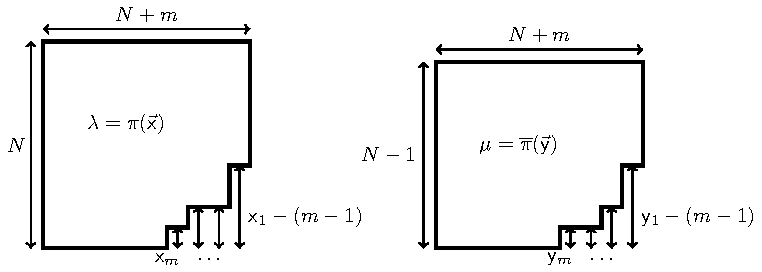
\includegraphics[width=.8\textwidth]{../assets/1305/fig_pi_of_x.pdf}
	\caption{Left: Young diagram of $\pi(\vec{\mathsf{x}})$ defined by
	\eqref{eq:pi_maps_1}--\eqref{eq:pi_maps_2}.
	The column lengths of the defect are $\mathsf{x}_j-(m-j)$.
	Right: Young diagram of $\overline\pi(\vec{\mathsf{y}})$.
	Observe that
	$\lambda=\pi(\vec{\mathsf{x}})$ and
	$\overline\pi(\vec{\mathsf{y}})$ differ only by
	adding the first row.}	\label{fig:pi_of_x}
\end{figure}

\begin{Lemma}	\label{lemma:interlacing}
	For any $\vec{\mathsf{x}},\vec{\mathsf{y}}\in \mathbb{W}_m(N)$,
	we have $\overline\pi(\vec{\mathsf{y}})\prec \pi(\vec{\mathsf{x}})$
	if and only if $\mathsf{y}_i=\mathsf{x}_i$ or $\mathsf{y}_i=\mathsf{x}_i-1$
	for all $i=1,\dots,m $.
\end{Lemma}
\begin{proof}
	Straightforward verification.
\end{proof}

In the rest of this section we
fix arbitrary $\vec{\mathsf{x}},\vec{\mathsf{y}}\in \mathbb{W}_m$ and
compute the limit of
$\Lambda^{N}_{N-1}(\pi(\vec{\mathsf{x}}),\overline\pi(\vec{\mathsf{y}}))$
\eqref{eq:traditional_links_Lambda}
under principal
specialization $x_j=t^{j-1}$
as $N\to+\infty$. Clearly, for sufficiently large $N$ the
partitions
$\pi(\vec{\mathsf{x}}),\overline\pi(\vec{\mathsf{y}})$
are well-defined.
We will show that this limit is equal
to the Markov kernel $\Upsilon_m(\vec{\mathsf{x}},\vec{\mathsf{y}})$
defined by~\eqref{eq:intro_Upsilon}.

Throughout the computation we adopt the convention
that
$\lambda=\pi(\vec{\mathsf{x}})$, $\mu=\overline\pi(\vec{\mathsf{y}})$.

\subsection{Initial Markov kernel}\label{sub:computation_initial_formula}

Our starting point is the formula for
$\Lambda^{N}_{N-1}(\pi(\vec{\mathsf{x}}),\overline\pi(\vec{\mathsf{y}}))$, see
\eqref{eq:traditional_links_Lambda},
under the principal
specialization $x_j=t^{j-1}$, which takes the form (where $\mu\prec\lambda$):
\begin{gather}
	\nonumber
		\Lambda^{N}_{N-1}(\lambda,\mu)
		=
		\psi_{\lambda/\mu}(q,t)\hspace{1pt} x_N^{|\lambda|-|\mu|}\hspace{1pt}
		\frac{
		P_\mu(x_1,\dots,x_{N-1} \mid q,t )
		}
		{P_\lambda(x_1,\dots,x_N \mid q,t)}
		\\
		\nonumber
\hphantom{\Lambda^{N}_{N-1}(\lambda,\mu)}{}
=
		\psi_{\lambda/\mu}
		(q,t)\hspace{1pt}
		t^{(N-1)(|\lambda|-|\mu|)}\hspace{1pt}
		\frac{P_\mu\big(1,t,\dots,t^{N-2}\mid q,t \big)}{P_\lambda\big(1,t,\dots,t^{N-2},t^{N-1}\mid q,t\big)}
		\\
		\nonumber
\hphantom{\Lambda^{N}_{N-1}(\lambda,\mu)}{}
=
		t^{(N-1)(|\lambda|-|\mu|)}
		\prod_{1\le i<j\le N-1}
		\frac{\mathsf{f}\big(q^{\mu_i-\mu_j}t^{j-i}\big)\hspace{1pt}
		\mathsf{f}(q^{\lambda_i-\lambda_{j+1}}t^{j-i})}
		{\mathsf{f}\big(q^{\lambda_i-\mu_j}t^{j-i}\big)\hspace{1pt}
		\mathsf{f}\big(q^{\mu_i-\lambda_{j+1}}t^{j-i}\big)}
		\\
\hphantom{\Lambda^{N}_{N-1}(\lambda,\mu)=}{}
\times
		t^{n(\mu)}\prod_{\square\in \mu}
		\frac{1-q^{a'(\square)}t^{N-1-l'(\square)}}
		{1-q^{a(\square)}t^{l(\square)+1}}
		t^{-n(\lambda)}
		\prod_{\square\in \lambda}
		\frac
		{1-q^{a(\square)}t^{l(\square)+1}}
		{1-q^{a'(\square)}t^{N-l'(\square)}}.		\label{eq:initial_formula}
\end{gather}
Here we used
\eqref{eq:principal_spec} and
\eqref{eq:psi_Pieri}.
Our next steps are devoted to
taking the limit as
$N\to+\infty$
in various parts of the product~\eqref{eq:initial_formula}.

\subsection[Power of t]{Power of $\boldsymbol{t}$}

Let us first consider the overall power of $t$
in \eqref{eq:initial_formula}
which is equal to
$t^{(N-1)(|\lambda|-|\mu|)+n(\mu)-n(\lambda)}$.
Our aim is to express quantities
depending on $\lambda$, $\mu$ through
$\vec{\mathsf{x}}$, $\vec{\mathsf{y}}$.
Adopt the convention
$\mathsf{x}_0=N+m$,
$\mathsf{y}_0=N+m-1$,
$\mathsf{x}_{m+1}=\mathsf{y}_{m+1}=-1$,
so that
\begin{equation*}
	N+m-\mathsf{x}_1-1=\mathsf{x}_0-\mathsf{x}_1-1,\qquad
	N+m-\mathsf{y}_1-2=\mathsf{y}_0-\mathsf{y}_1-1.
\end{equation*}
We have from \eqref{eq:pi_maps_multiplicative_notation}:
\begin{gather*}
	|\lambda|-|\mu|	=
	\sum_{i=0}^{m}
	(N+i)
	(
	( \mathsf{x}_{m-i}-\mathsf{x}_{m-i+1}-1 )-
	( \mathsf{y}_{m-i}-\mathsf{y}_{m-i+1}-1)
)
	\\
\hphantom{|\lambda|-|\mu|}{}
=
	\sum_{i=0}^{m}
	(N+i)
	(
	( \mathsf{x}_{m-i}-\mathsf{x}_{m-i+1} )-
	( \mathsf{y}_{m-i}-\mathsf{y}_{m-i+1} )
)
	\\
\hphantom{|\lambda|-|\mu|}{}
=
	N\sum_{i=0}^{m}
	(
	( \mathsf{x}_{m-i}-\mathsf{x}_{m-i+1} )-
	( \mathsf{y}_{m-i}-\mathsf{y}_{m-i+1} )
	)\\
\hphantom{|\lambda|-|\mu|=}{}
	+
	\sum_{i=0}^{m}i
	(
	( \mathsf{x}_{m-i}-\mathsf{x}_{m-i+1} )-
	( \mathsf{y}_{m-i}-\mathsf{y}_{m-i+1})
	)
	\\
\hphantom{|\lambda|-|\mu|}{}
=
	N+m+
	|\vec {\mathsf{y}}|-|\vec{\mathsf{x}}|.
\end{gather*}
Moreover, from
\eqref{eq:n_lambda_notation} and \eqref{eq:pi_maps_multiplicative_notation}
we have
\begin{gather}
	\nonumber
	n(\mu)-n(\lambda)
	=
	\sum_{j=0}^{m}
	(N+m-j)
	\left[
		\binom{\mathsf{y}_0-\mathsf{y}_{j+1}-(j+1)}2-
		\binom{\mathsf{y}_0-\mathsf{y}_{j}-j}2
	\right]
	\\
\hphantom{n(\mu)-n(\lambda)=}{}
-
	\sum_{j=0}^{m}
	(N+m-j)
	\left[
		\binom{\mathsf{x}_0-\mathsf{x}_{j+1}-(j+1)}2-
		\binom{\mathsf{x}_0-\mathsf{x}_{j}-j}2
	\right]
\nonumber\\
\hphantom{n(\mu)-n(\lambda)}{}
=
	-(N-1)(N+m)
	-\binom{m}{2}
	+|\vec{\mathsf{x}}|\nonumber\\
\hphantom{n(\mu)-n(\lambda)=}{}
+
	\frac12
	\sum_{i=1}^{m}
	(\mathsf{y}_i-\mathsf{x}_i)(\mathsf{x}_i+\mathsf{y}_i+3+2i-2m-2N).
\label{eq:newlabel}
\end{gather}
Indeed, the coefficients
by $\mathsf{x}_i$, $\mathsf{x}_i^2$, $\mathsf{y}_i$, $\mathsf{y}_i^2$, $1\le i\le m$, in the right-hand side of~\eqref{eq:newlabel}
are, respectively,
\begin{equation*}
	N - i + m - \frac{1}{2}
	,\
	-\frac{1}{2}
	,\
	-N + i - m + \frac32
	,\
	\frac{1}{2},
\end{equation*}
which are the same as in the left-hand side.
The free term in the left-hand side is
$-\binom m2+m-N^2-(m-2)N$,
which is readily matched to the free term in the
right-hand side by virtue of
our conventions about
$\mathsf{x}_0$, $\mathsf{y}_0$, $\mathsf{x}_{m+1}$, $\mathsf{y}_{m+1}$.

Let us further simplify the left-hand side of
\eqref{eq:newlabel}.
The $i$-th term in this sum
is rewritten as
\begin{gather*}
	\frac12(\mathsf{y}_i-\mathsf{x}_i)(\mathsf{x}_i+\mathsf{y}_i+3+2i-2m-2N)\\
\qquad{}
	=
	-(N-1)(\mathsf{y}_i-\mathsf{x}_i)
	+
	\frac12(\mathsf{y}_i-\mathsf{x}_i)(-\mathsf{x}_i+\mathsf{y}_i+1)
	+
	(\mathsf{y}_i-\mathsf{x}_i)(\mathsf{x}_i-m+i).
\end{gather*}
Since $\mathsf{y}_i-\mathsf{x}_i$ is equal to $0$ or $-1$,
the quantity
$(\mathsf{y}_i-\mathsf{x}_i)(-\mathsf{x}_i+\mathsf{y}_i+1)$
is identically zero.
Thus, we have
\begin{align*}
	n(\mu)-n(\lambda)=
	-(N-1)(N+m+|\vec{\mathsf{y}}|-|\vec{\mathsf{x}}|)
	+|\vec{\mathsf{x}}|-\binom m2
	+\sum_{i=1}^{m}
	(\mathsf{x}_{i}-m+i)(\mathsf{y}_{i}-\mathsf{x}_{i}).
\end{align*}
We see that
the $N$-dependent terms
in
$(N-1)(|\lambda|-|\mu|)+n(\mu)-n(\lambda)$
cancel out, and the overall
factor containing the
power of $t$
in
$\Lambda^{N}_{N-1}(\pi(\vec{\mathsf{x}}),\overline\pi(\vec{\mathsf{y}}))$
has the form
\begin{equation*}%\label{eq:power_of_t_final}
	t^{-\binom m2+|\vec{\mathsf{x}}|
	+\sum_{i=1}^{m}
	(\mathsf{x}_{i}-m+i)(\mathsf{y}_{i}-\mathsf{x}_{i})}.
\end{equation*}

\subsection{Coarms and colegs}
Addressing the factors in
\eqref{eq:initial_formula}
containing coarms and colegs of $\lambda$ and $\mu$,
we obtain using \eqref{eq:arms_legs}:
\begin{equation*}
	\prod_{\square\in \lambda}\big(1-q^{a'(\square)}t^{N-l'(\square)}\big)
	=
	\prod_{i=1}^{N}
	\prod_{j=1}^{\lambda_i}
	\big(1-q^{j-1}t^{N-i+1}\big)
	=
	\prod_{i=1}^{N}
	\big(t^{N+1-i};q\big)_{\lambda_i}.
\end{equation*}
This product is in the denominator, and a similar
factor
$\prod_{i=1}^{N-1}
\big(t^{N-i};q\big)_{\mu_i}$
appears in the numerator.
Let us show that the contribution coming from
coarms and colegs goes to one, that is,%
\begin{equation}
	\label{eq:coarm_coleg_result}
	\lim_{N\to+\infty}
	\frac{\prod_{i=1}^{N-1}
	\big(t^{N-i};q\big)_{\mu_i}}
	{\prod_{i=1}^{N}
	\big(t^{N+1-i};q\big)_{\lambda_i}}=1.
\end{equation}
To see this, observe that
$\mu_{i}-\lambda_{i+1}$ for all $i=1,\dots,N-1 $ is a nonnegative integer
which does not grow with $N$ as long as $N-i$ is fixed,
see~\eqref{eq:pi_maps_multiplicative_notation}. Therefore,
\begin{gather*}
	\frac{\big(t^{N-i};q\big)_{\mu_i}}{\big(t^{N+1-(i+1)};q\big)_{\lambda_{i+1}}}=
	\frac{\big(t^{N-i};q\big)_{\mu_i}}{\big(t^{N-i};q\big)_{\lambda_{i+1}}}\\
\hphantom{\frac{\big(t^{N-i};q\big)_{\mu_i}}{\big(t^{N+1-(i+1)};q\big)_{\lambda_{i+1}}}}{}
=
	\big(1-t^{N-i}q^{\lambda_{i+1}}\big)\big(1-t^{N-i}q^{\lambda_{i+1}+1}\big)\cdots\big(1-t^{N-i}q^{\mu_i-1}\big) ,
\end{gather*}
where the product in the right-hand side is finite. Since $\lambda_{i+1}$ and $\mu_i$ go to infinity
as $N\to\infty$, this product converges to~$1$.
There is one more factor in the denominator of~\eqref{eq:coarm_coleg_result},
namely,
\begin{equation*}
	\frac{1}{\big(t^N;q\big)_{\lambda_1}}=
	\frac{\big(t^Nq^{N+m};q\big)_\infty}{\big(t^N;q\big)_\infty}.
\end{equation*}
This factor also goes to $1$ as $N\to+\infty$,
and so the limit~\eqref{eq:coarm_coleg_result} is established.

\subsection{Arms and legs}

We now consider the product
in \eqref{eq:initial_formula}
involving arms and legs:
\begin{equation}
	\label{eq:arm_leg_product_initial}
	\prod_{\square\in \mu}
	\frac{1}
	{1-q^{a(\square)}t^{l(\square)+1}}
	\prod_{\square\in \lambda}
	\bigl(1-q^{a(\square)}t^{l(\square)+1}\bigr).
\end{equation}
Recall the notation
$\lambda=\pi(\vec{\mathsf{x}})$,
$\mu=\overline\pi(\vec{\mathsf{y}})$, see~\eqref{eq:pi_maps_multiplicative_notation}.
Observe that the Young diagrams
$\lambda=\pi(\vec{\mathsf{x}})$ and
$\overline\pi(\vec{\mathsf{y}})$ differ only by
adding the first row (cf.\ Figure~\ref{fig:pi_of_x}).
For each box $\square$ in the first row of $\lambda$, the quantity
$l(\square)$ is of order $N$, and so
$1-q^{a(\square)}t^{l(\square)+1}$ is close to~$1$
for large $N$.
Therefore, the product
\eqref{eq:arm_leg_product_initial}
has the same limit as
\begin{equation}	\label{eq:arm_leg_product_proof_1}
	\prod_{\square\in \overline\pi(\vec{\mathsf{y}})}
	\frac{1}
	{1-q^{a(\square)}t^{l(\square)+1}}
	\prod_{\square\in \overline\pi(\vec{\mathsf{x}})}
	\bigl(1-q^{a(\square)}t^{l(\square)+1}\bigr).
\end{equation}

\begin{Proposition}	\label{prop:arm_leg_main_result}
	As $N\to+\infty$, the product \eqref{eq:arm_leg_product_proof_1}
	converges to
	\begin{equation*}%\label{eq:arm_leg_limit_thing}
		\frac{V_{t,q}(\vec{\mathsf{y}})}{V_{t,q}(\vec{\mathsf{x}})}
		\prod_{i=1}^{m}
		\big( 1-q^{m-i}t^{\mathsf{x}_i-m+i}\mathbf{1}_{\mathsf{y}_i=\mathsf{x}_i-1} \big),
	\end{equation*}
	where $V_{t,q}$ is the $(t,q)$-Vandermonde given by \eqref{eq:V_tq}.
\end{Proposition}
\begin{proof}
	Recall the notation
	for the
	$(q,t)$-deformed hook polynomials
	\cite[formulas~(VI.8.1) and (VI.8.1$'$)]{Macdonald1995}:
	\begin{equation*}
		c_\nu(q,t)=
		\prod_{\square\in \nu}\bigl(1-q^{a(\square)}t^{l(\square)+1}\bigr),\qquad
		c'_\nu(q,t)=
		\prod_{\square\in \nu}\bigl(1-q^{a(\square)+1}t^{l(\square)}\bigr),
	\end{equation*}
	and observe that $c_\nu(q,t)=c'_{\nu'}(t,q)$, where $\nu'$ is the
	transposed Young diagram.
	Note that, in multiplicative notation,
	\begin{gather*}
		\overline\pi(\vec{\mathsf{x}})'=
		(N-1)^{N}
		(N-1-\mathsf{x}_m)
		(N-1-\mathsf{x}_{m-1}+1)
		(N-1-\mathsf{x}_{m-2}+2)
		\cdots\\
\hphantom{\overline\pi(\vec{\mathsf{x}})'=}{}
\times (N-1-\mathsf{x}_{1}+m-1)
	\end{gather*}
	and similarly for $\overline\pi(\vec{\mathsf{y}})'$,
	see Figure~\ref{fig:pi_of_x}.
	Adopt the convention
	$\mathsf{x}_{m+j}=\mathsf{y}_{m+j}
	=-j$ for $j=1,2,\dots $.
	Then we may shift the indices $j$ to encode the string $\overline\pi(\vec{\mathsf{x}})'$
	as
	$\overline\pi(\vec{\mathsf{x}})'_j=N+j-1-\mathsf{x}_{m-j}$,
	where $-N\le j\le m-1$, and similarly for $\vec{\mathsf{y}}$.
	The arm and leg lengths do not change under this shifting.
	This shift allows to directly refer to a known identity, the first one in
	\cite[Proposition~3.2]{kaneko1996q}, and write
	\begin{gather*}
		c_{\overline\pi(\vec{\mathsf{x}})}(q,t)
		=
		c'_{\overline\pi(\vec{\mathsf{x}})'}(t,q)
		\\
\hphantom{c_{\overline\pi(\vec{\mathsf{x}})}(q,t)}{}
=
		\frac{(t;t)_{\infty}^{N+m}}
		{
			\prod_{j=-N}^{m-1}
			\big(t^{N+j-\mathsf{x}_{m-j}}q^{m-1-j};t\big)_{\infty}
		}
		\prod_{-N\le i<j\le m-1}
		\frac{\big(q^{j-i}t^{i-j-\mathsf{x}_{m-i}+\mathsf{x}_{m-j}+1};t\big)_{\infty}}
		{\big(q^{j-i-1}t^{i-j-\mathsf{x}_{m-i}+\mathsf{x}_{m-j}+1};t\big)_{\infty}}
		\\
\hphantom{c_{\overline\pi(\vec{\mathsf{x}})}(q,t)}{}
		=
		\frac{(t;t)_{\infty}^{N+m}}
		{
			\prod_{j=-N}^{m-1}
			\big(t^{N+j-\mathsf{x}_{m-j}}q^{m-1-j};t\big)_{\infty}
		}
		\prod_{-N\le i<j\le -1}
		\frac{\big(q^{j-i}t;t\big)_{\infty}}
		{\big(q^{j-i-1}t;t\big)_{\infty}}
		\\
\hphantom{c_{\overline\pi(\vec{\mathsf{x}})}(q,t)=}{}
\times
		\prod_{\substack{-N\le i\le -1 \\ 0\le j\le m-1}}
		\frac{\big(q^{j-i}t^{-j+\mathsf{x}_{m-j}+1};t\big)_{\infty}}
		{\big(q^{j-i-1}t^{-j+\mathsf{x}_{m-j}+1};t\big)_{\infty}}
		\underbrace{
		\prod_{1\le i<j\le m}
		\frac{\big(q^{j-i}t^{i-j-\mathsf{x}_{j}+\mathsf{x}_{i}+1};t\big)_{\infty}}
		{\big(q^{j-i-1}t^{i-j-\mathsf{x}_{j}+\mathsf{x}_{i}+1};t\big)_{\infty}}}
		_{1/V_{t,q}(\vec{\mathsf{x}})}.
	\end{gather*}
	Therefore,
	the product \eqref{eq:arm_leg_product_proof_1}
	becomes
	\begin{gather*}
		\frac{c_{\overline\pi(\vec{\mathsf{x}})}(q,t)}
		{c_{\overline\pi(\vec{\mathsf{y}})}(q,t)}
		=
		\frac{V_{t,q}(\vec{\mathsf{y}})}
		{V_{t,q}(\vec{\mathsf{x}})}
			\prod_{j=1}^{m}
		\frac{
			\big(t^{N+m-j-\mathsf{y}_{j}}q^{j-1};t\big)_{\infty}
		}
		{
			\big(t^{N+m-j-\mathsf{x}_{j}}q^{j-1};t\big)_{\infty}
		}\\
\hphantom{\frac{c_{\overline\pi(\vec{\mathsf{x}})}(q,t)}
		{c_{\overline\pi(\vec{\mathsf{y}})}(q,t)}=}{}
\times
		\prod_{j=1}^{m}
		\prod_{i=-N}^{-1}
		\frac{\big(q^{m-j-i}t^{j-m+\mathsf{x}_{j}+1};t\big)_{\infty}}
		{\big(q^{m-j-i-1}t^{j-m+\mathsf{x}_{j}+1};t\big)_{\infty}}
		\frac
		{\big(q^{m-j-i-1}t^{j-m+\mathsf{y}_{j}+1};t\big)_{\infty}}
		{\big(q^{m-j-i}t^{j-m+\mathsf{y}_{j}+1};t\big)_{\infty}}.
	\end{gather*}
	The first product over $1\le j\le m$
	converges to $1$ as $N\to+\infty$
	thanks to the presence of $t^N$.
	In the second product over $1\le j\le m$, the terms
	where $\mathsf{y}_j=\mathsf{x}_j$ are simply equal to $1$.
	When $\mathsf{y}_j=\mathsf{x}_j-1$, we have
	\begin{gather*}
		\prod_{i=-N}^{-1}
		\frac{\big(q^{m-j-i}t^{j-m+\mathsf{x}_{j}+1};t\big)_{\infty}}
		{\big(q^{m-j-i-1}t^{j-m+\mathsf{x}_{j}+1};t\big)_{\infty}}
		\frac
		{\big(q^{m-j-i-1}t^{j-m+\mathsf{x}_{j}};t\big)_{\infty}}
		{\big(q^{m-j-i}t^{j-m+\mathsf{x}_{j}};t\big)_{\infty}}
	\\
\qquad{}	 =
		\prod_{i=1}^{N}
		\frac{1-q^{m-j+i-1}t^{j-m+\mathsf{x}_{j}}}
		{1-q^{m-j+i}t^{j-m+\mathsf{x}_{j}}}
	 =
		\frac{1-q^{m-j}t^{j-m+\mathsf{x}_{j}}}
		{1-q^{m-j+N}t^{j-m+\mathsf{x}_{j}}},
	\end{gather*}
	and the $N\to+\infty$ limit of this expression is
	$1-q^{m-j}t^{\mathsf{x}_{j}-m+j}$.
	This completes the proof.
\end{proof}

\subsection{Pieri coefficient}

It remains to consider the $N\to+\infty$ limit of the Pieri
coefficient $\psi_{\lambda/\mu}(q,t)$
entering \eqref{eq:initial_formula}.
Recall the convention
$\mathsf{x}_{m+j}=\mathsf{y}_{m+j}
=-j$ for $j=1,2,\dots $,
and encode (shifting the indices)
\begin{equation*}
	\lambda'_i=\pi(\vec{\mathsf{x}})'_i=N+i-\mathsf{x}_{m-i},
	\qquad
	\mu'_j=\overline\pi(\vec{\mathsf{y}})'_j=N-1+j-\mathsf{y}_{m-j}.
\end{equation*}
We can now use
the well-known duality
\cite[proof of formula~(6.24)]{Macdonald1995}
\begin{equation*}
	\psi_{\lambda/\mu}(q,t)=
	\psi'_{\lambda'/\mu'}(t,q),
\end{equation*}
and obtain from~\eqref{eq:psi_prime_Pieri}:
\begin{gather*}
	\psi'_{\lambda'/\mu'}(t,q)
	=
	\prod_{\substack{-N\le i<j\le m-1
	\\
	\lambda'_{i}=\mu'_{i},\, \lambda'_{j}=\mu'_{j}+1}}
	\frac{\big(1-t^{\mu'_{i}-\mu'_{j}} q^{j-i-1}\big)\big(1-t^{\lambda'_{i}-\lambda'_{j}} q^{j-i+1}\big)}
	{\big(1-t^{\mu'_{i}-\mu'_{j}} q^{j-i}\big)\big(1-t^{\lambda'_{i}-\lambda'_{j}} q^{j-i}\big)}
	\\
\hphantom{\psi'_{\lambda'/\mu'}(t,q)=}{}
=
	\prod_{\substack{-N\le i<j\le m-1
	\\
	\mathsf{y}_{m-i}=\mathsf{x}_{m-i}-1,\\
	\mathsf{y}_{m-j}=\mathsf{x}_{m-j}}}
	\frac{\big(1-t^{i-j+\mathsf{y}_{m-j}-\mathsf{y}_{m-i}}
	q^{j-i-1}\big)
	\big(1-t^{i-j+\mathsf{x}_{m-j}-\mathsf{x}_{m-i}} q^{j-i+1}\big)}
	{\big(1-t^{i-j+\mathsf{y}_{m-j}-\mathsf{y}_{m-i}} q^{j-i}\big)
	\big(1-t^{i-j+\mathsf{x}_{m-j}-\mathsf{x}_{m-i}} q^{j-i}\big)}.
\end{gather*}
Split the product over $i<j$ into three parts.
The first part with $-N\le i<j\le -1$
cancels out and is equal to $1$
since
we have $\mathsf{y}_{m-i}=\mathsf{x}_{m-i}$ for all $-N\le i\le -1$.
The second part
with $-N\le i\le -1$ and $0\le j\le m-1$ is also equal to $1$ for the same reason.
The third part with $0\le i<j\le m-1$ equals
\begin{equation}
	\label{eq:psi_prime_in_limit}
	\prod_{\substack{1\le i<j\le m
	\\
	\mathsf{y}_{i}=\mathsf{x}_{i}
	,\,
	\mathsf{y}_{j}=\mathsf{x}_{j}-1}}
	\frac{\big(1-t^{i-j+\mathsf{y}_{i}-\mathsf{y}_{j}}
	q^{j-i-1}\big)
	\big(1-t^{i-j+\mathsf{x}_{i}-\mathsf{x}_{j}} q^{j-i+1}\big)}
	{\big(1-t^{i-j+\mathsf{y}_{i}-\mathsf{y}_{j}} q^{j-i}\big)
	\big(1-t^{i-j+\mathsf{x}_{i}-\mathsf{x}_{j}} q^{j-i}\big)},
\end{equation}
which is independent of $N$. Note that
\eqref{eq:psi_prime_in_limit} is equal to a Pieri coefficient
$\psi'_{(\vec{\mathsf{x}}-\delta_m)/(\vec{\mathsf{y}}-\delta_m)}(t,q)$,
where $\delta_m=(m-1,m-2,\dots,2,1,0)$ is the
staircase partition.

\subsection{Final result}

Putting together all the computations from this section, we see that the
$N\to+\infty$ limit of the Markov kernel $\Lambda^{N}_{N-1}(\pi(\vec{\mathsf{x}}),
\overline\pi(\vec{\mathsf{y}}))$ is the Markov kernel (on $\mathbb{W}_m$)
of the Macdonald noncolliding walks with the absorbing wall at zero:
\begin{gather}
	\nonumber
	\Upsilon_m(\vec{\mathsf{x}},\vec{\mathsf{y}}) =
	t^{-\binom m2+|\vec{\mathsf{x}}|
	+\sum_{i=1}^{m}
	(\mathsf{x}_{i}-m+i)(\mathsf{y}_{i}-\mathsf{x}_{i})}	
	\hspace{1pt}
	\frac{V_{t,q}(\vec{\mathsf{y}})}{V_{t,q}(\vec{\mathsf{x}})}
	\hspace{1pt}
	\psi'_{(\vec{\mathsf{x}}-\delta_m)/(\vec{\mathsf{y}}-\delta_m)}(t,q)
	\\
\hphantom{\Upsilon_m(\vec{\mathsf{x}},\vec{\mathsf{y}})=}{}	
\times
	\prod_{i=1}^{m}
	\big( 1-q^{m-i}t^{\mathsf{x}_i-m+i}\mathbf{1}_{\mathsf{y}_i=\mathsf{x}_i-1}\big)\nonumber
	\\
	\nonumber
\hphantom{\Upsilon_m(\vec{\mathsf{x}},\vec{\mathsf{y}})}{}	
=
	t^{-\binom m2}	
	\hspace{1pt}
	\prod_{1\le i<j\le m}
	\frac
	{
		\big(q^{j-i} t^{\mathsf{x}_i-\mathsf{x}_j-j+i+1};t\big)_{\infty}
		\big( q^{j-i-1}t^{\mathsf{y}_i-\mathsf{y}_j-j+i+1};t \big)_{\infty}
	}
	{
		\big( q^{j-i-1}t^{\mathsf{x}_i-\mathsf{x}_j-j+i+1};t \big)_{\infty}
		\big(q^{j-i} t^{\mathsf{y}_i-\mathsf{y}_j-j+i+1};t\big)_{\infty}
	}
	\\
\hphantom{\Upsilon_m(\vec{\mathsf{x}},\vec{\mathsf{y}})=}{}	\times
\nonumber
	\prod_{\substack{1\le i<j\le m
	\\
	\mathsf{y}_{i}=\mathsf{x}_{i}
	,\,
	\mathsf{y}_{j}=\mathsf{x}_{j}-1}}
	\frac{\big(1-t^{i-j+\mathsf{x}_{i}-\mathsf{x}_{j}+1}
	q^{j-i-1}\big)
	\big(1-t^{i-j+\mathsf{x}_{i}-\mathsf{x}_{j}} q^{j-i+1}\big)}
	{\big(1-t^{i-j+\mathsf{x}_{i}-\mathsf{x}_{j}+1} q^{j-i}\big)
	\big(1-t^{i-j+\mathsf{x}_{i}-\mathsf{x}_{j}} q^{j-i}\big)}
	\\
\hphantom{\Upsilon_m(\vec{\mathsf{x}},\vec{\mathsf{y}})=}{}	\times
	\prod_{i\colon \mathsf{y}_i=\mathsf{x}_i}
	t^{\mathsf{x}_i}
	\prod_{i\colon \mathsf{y}_i=\mathsf{x}_i-1}
	\big(t^{m-i}-q^{m-i}t^{\mathsf{x}_i}\big)
	.\label{eq:Upsilon_final_formula}
\end{gather}
The second expression is obtained by rewriting the
powers of $t$, and expanding the notation of~$V_{t,q}$ and~$\psi'$.
This completes the proof of Theorem~\ref{thm:Macdonald_noncolliding_intro}.
\section*{Editable transcription of original figure labels}
\noindent This is a faithful transcription of the literal printed labels, separate from the native author TeX. The original figure panels above remain unchanged. Positions below identify labels and do not infer any unprinted entries. Source asset and panel boundaries are recorded in figure-label-transcription-r001.json.
\begin{description}
\item[Original Figure 1, fig\_Young\_d.pdf.] Top horizontal coordinate arrow: $j$. Left downward coordinate arrow: $i$. Marked box: $(3,2)$. Right row labels, from top: $\lambda_1$, $\lambda_2$, $\lambda_3$, $\vdots$. Bottom column labels, from left: $\lambda'_1$, $\lambda'_2$, $\lambda'_3$, $\cdots$.
\item[Original Figure 2, fig\_pi\_of\_x.pdf, left panel.] Center: $\lambda=\pi(\vec{x})$. Top horizontal size arrow: $N+m$. Left vertical size arrow: $N$. Bottom defect labels, from left: $x_m$, $\ldots$. Right vertical defect size: $x_1-(m-1)$.
\item[Original Figure 2, fig\_pi\_of\_x.pdf, right panel.] Center: $\mu=\overline{\pi}(\vec{y})$. Top horizontal size arrow: $N+m$. Left vertical size arrow: $N-1$. Bottom defect labels, from left: $y_m$, $\ldots$. Right vertical defect size: $y_1-(m-1)$.
\end{description}

\begin{thebibliography}{99}
\bibitem[2]{Borodin2010Schur}
Borodin A., Schur dynamics of the {S}chur processes, \href{https://doi.org/10.1016/j.aim.2011.06.038}{\textit{Adv. Math.}}
 \textbf{228} (2011), 2268--2291, \href{https://arxiv.org/abs/1001.3442}{arXiv:1001.3442}.

\bibitem[3]{BorodinCorwin2011Macdonald}
Borodin A., Corwin I., Macdonald processes, \href{https://doi.org/10.1007/s00440-013-0482-3}{\textit{Probab. Theory Related
 Fields}} \textbf{158} (2014), 225--400, \href{https://arxiv.org/abs/1111.4408}{arXiv:1111.4408}.

\bibitem[4]{BorFerr2008DF}
Borodin A., Ferrari P.L., Anisotropic growth of random surfaces in {$2+1$}
 dimensions, \href{https://doi.org/10.1007/s00220-013-1823-x}{\textit{Comm. Math. Phys.}} \textbf{325} (2014), 603--684,
 \href{https://arxiv.org/abs/0804.3035}{arXiv:0804.3035}.

\bibitem[6]{borodin2016representations}
Borodin A., Olshanski G., Representations of the infinite symmetric group,
 \textit{Cambridge Studies in Advanced Mathematics}, Vol.~160, \href{https://doi.org/10.1017/CBO9781316798577}{Cambridge
 University Press}, Cambridge, 2017.

\bibitem[15]{kaneko1996q}
Kaneko J., {$q$}-{S}elberg integrals and {M}acdonald polynomials, \href{https://doi.org/10.24033/asens.1749}{\textit{Ann.
 Sci. \'{E}cole Norm. Sup.~(4)}} \textbf{29} (1996), 583--637.

\bibitem[20]{Macdonald1995}
Macdonald I.G., Symmetric functions and {H}all polynomials, 2nd~ed., \textit{Oxford Math. Monogr.}, The Clarendon Press, Oxford University Press, New
 York, 1995.

\end{thebibliography}
\end{document}
